\documentclass[10pt,a4paper]{article}

\usepackage{fullpage}
\usepackage{wrapfig}
\usepackage{lipsum}
\usepackage{hyperref}
\usepackage{cleveref}
\usepackage{tikz}
\usepackage{float}
\usepackage{comment}

\DeclareGraphicsExtensions{.pdf,.png,.jpg}

\begin{document}
\title{WebApp Group 34 Milestone Report}
\author{
  Han, Qiao\\
  \and
  Chabierski, Piotr\\
  \and
  Smith, Bradley\\
  \and
  Cingillioglu, Nuri\\
}

\maketitle

\section{Group Structure and Work Division}

\noindent
We divided our group responsibilities based on our individual strengths. Han has done extensive development work on both server and client side applications in past internships and part time jobs and hence is the most suitable candidate for the role of group leader. The group leader is responsible for guiding the choices of technology together with ensuring a schedule for the timely completion of the project. In addition, he is also responsible for managing the team during evaluations of the project requirements and the suitability of different technology stacks in fulfilling our design goals.
\\
\\
\noindent
More specifically, our team members are initially in charge of working on following areas.

\begin{enumerate}
  \item Client-side presentation - Nuri
  \item Client-side interaction - Nuri / Han
  \item Server-side processing - Bradley / Piotr / Han
  \item Database set-up - Bradley / Piotr
\end{enumerate}

\noindent
As we progress, we believe we will work on different parts of the project from this initial assignment so that everyone will get a holistic understanding of the full stack web development process.


\section{Choice of Implementation Languages}
Although the frontend has to be written in HTML, CSS, and Javascript, we have considered a wide variety of web development frameworks, ranging from full blown MVC frameworks such as AngularJS, MeteorJS, and Django templates, to minimalistic libraries such as jQuery, Backbone.js, and HTML5 Boilerplate. As the team is relatively new to web development, we decided to use frameworks that more closely represent the fundamental DOM layout to enhance our understanding. This means that HTML5 Boilerplate is a good choice because it consolidates the best practices of using modern web technologies without adding extra layers of abstraction. In addition, we have chosen to use the Bootstrap framework to enhance the visual presentation of our web app. Lastly, we decided to separate our data models from the views by fetching data asynchronously as JSON objects from our backend using RESTful APIs. Using RESTful APIs allows for easy integration with mobile clients while using JSON as the data format allows for transfer of rich data structures like nested objects and arrays.
\begin{comment}
  see also, closure, scala, dart, go, c++
\end{comment}
\\
\\
\noindent
We have picked a statically typed language, Java, as the implementation language for our backend. Although it may increase the amount of time needed to write our App, we believe the extra type safety combined with an active developer community makes it a good trade-off over other dynamically typed languages such as Python, node.js, and PHP. As most of us are familiar with Java, it is also easier to apply sound software design patterns that we have learnt over the course of our studies, such as singleton pattern or dependency injection/inversion. With the support of testing frameworks like JUnit and Mockito, we are able to provide good test coverage on our backend code base to ensure long term maintainability. This is especially important for our target market - enterprise web apps (see our App description). More generally, Java code is more habitable and allows for easier extension with its wide range of third party libraries. We also believe it will keep our options open going forward as it is very portable and platform independent.
\\
\\
\noindent
Lastly, we have decided to use Apache Tomcat as the web container and PostgreSQL as the database engine because they have been conveniently set up by CSG on lab machines.

\section{Description of our App}
Our project is a multi-user calendar App which allows users to, create/subscribe to calendars, create/join events and obtain feedback on who has signed up to their events. The App is targeted at volunteers for college events but can be easily extended for more general purposes.
\\
\\
\noindent
It has three main entity types: the users, the calendars and the events, and several relations between them, see \cref{sec:er} for more details. The idea came from a specific problem that we found occurring very often, namely people using emails to organise events and work out specifically who can attend or get a general idea of how many people to expect. This can lead to very inefficient communication and cause a variety of organisation hardships. Examples of such common problematic situation are events occurring so often that the people who are attending (volunteering) start to pay less attention to them, or events being so popular that they ends up being over subscribed and the organisers have to send a huge number of emails back to the people who didn't make it in time.
\\
\\
\noindent
We are creating our App while having these problems in mind and aim to come up with a system which could eliminate or ease some of them by grouping the related events into calendars and presenting them to user in an ordered manner.

\section{User Interactions} 
The basic idea is that there will be two types of users (per calendar), the administrators and the ordinary users (subscribers). They will both interact with the calendars in different ways and have various typical uses. Note that any user can create a calendar or join other calendars so these roles are not absolute.
\\
\\
\noindent
A subscriber of a calendar needs to be able to see calendar's events in a clear manner and easily access the details of an event, like time, location, duration and short description, together with a feedback on the interest about the event (number of people already registered to the event). Users also need the ability to sign up for the event they wish to attend (depending on the event this might be a strict attendance or a flexible one). In addition, users should be able to change between the calendars they are subscribed to and create a dynamically-customisable view including only the calendars that interest them at a particular time. The view would enable the users to preview the information about events occurring in a certain time interval (for example, in two weeks from the current date). Finally, all users of the App should be able to create calendars and gain administrator privilege on them. 
\\
\\
\noindent
The administrations of a calendar need extra abilities in addition to those of a subscriber. They will be able to create, modify details of and delete any event on their calendars along with the ability to see the number of people who have signed up and their identities. In addition, they can delete whole calendars and invite people to subscribe via an invite code which they can give out to anyone who may be interested. We are also looking into other ways that users may be invited to calendars.  
\\
\\
\noindent
Lastly, everyone will also be able to interact by registering and logging in to our App, see \cref{sec:fd} for user flow diagrams.

\appendix
\label{appendix}

\section{System Entities and Relations} 
\label{sec:er}
\begin{figure}[H]
\centerline{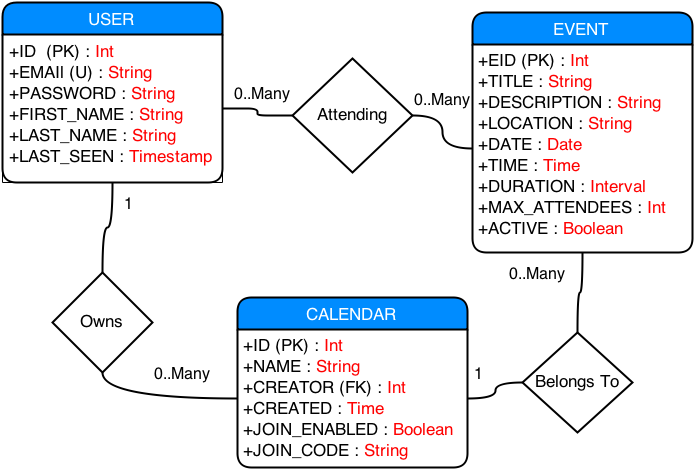
\includegraphics[scale=0.58,trim=0 0 100 0]{er}}
\caption{Entity Relation diagram with possible database layout}
\end{figure}
PK, FK and U stand for Primary Key, Foreign Key and Unique respectively. PK implies U.
\\
\\
\noindent
There is a relationship missing from this diagram, namely the subscriber relationship. Each of the relationships will be represented in the database as a table with ID to ID mappings between the two participants. The cardinality constraints can also be very easily added into the database to ensure that the data remains consistent. For example the \textbf{belongs to} relationship will be realised with a table with one column being the CID (Calendar Id) and the other being the EID (Event Id). The (CID,EID) pair will be the primary key.
\newpage
\section{User Interaction Diagrams}
\label{sec:fd}
\begin{figure}[H]
\centering
\begin{minipage}{.4\textwidth}
  \centering
  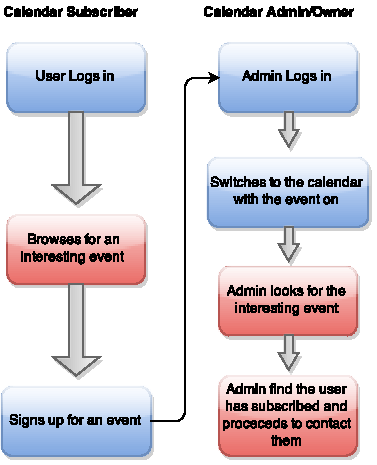
\includegraphics[width=1\linewidth]{user_event}
  \caption{Use flow of a user signing up}
\end{minipage}%
\begin{minipage}{.7\textwidth}
  \centering
  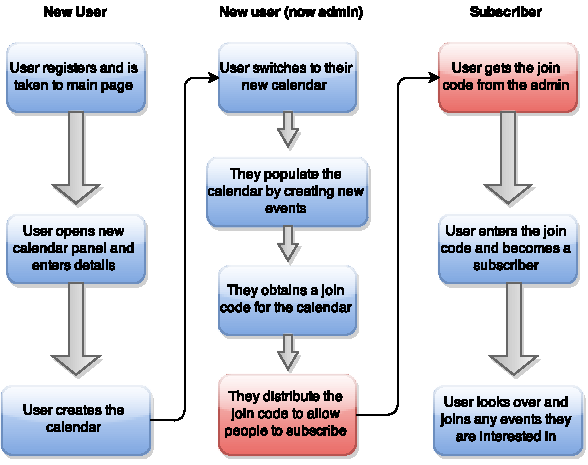
\includegraphics[width=0.9\linewidth]{calendar_user}
  \caption{Use flow of a new user creating a calendar}
\end{minipage}
\end{figure}
\noindent These diagrams show two typical use situations it which the user would interact with our WebApp. The blue boxes are explicit interactions with our App, where as the red boxes are events which require no explicit (but most likely some) interaction.

\end{document}
